\documentclass[%
	pdftex,
	oneside,        % One-sided print
	11pt,           % Font size
	parskip=half,   % The half of a line margin after line feeds
	headsepline,    % Line after header
	footsepline,    % Line after footer
	abstracton,     % Abstract headings
	USenglish,      % Written in English
	a4paper,        % Written on Din A4 paper
]{report}


\title{Knowledge based systems\\ Analysing the eligibility of a person for higher education using a Bayesian network}
\author{Lisa Mischer \& Frank Steiler\\ Interactive and knowledge based systems (T2INF4307)\\ DHBW Stuttgart\\ Contact: it12147@lehre.dhbw-stuttgart.de}
        
\usepackage[english]{babel}
\usepackage[english=british]{csquotes}
\usepackage[style=alphabetic,backend=biber,natbib=true]{biblatex}
\addbibresource{Documentation.bib}
\usepackage{graphicx}
\usepackage{setspace}
\usepackage{hyperref}
\usepackage{varioref}
\usepackage{chngcntr}
\usepackage{subcaption}
\usepackage[export]{adjustbox}[2011/08/13]
\usepackage{fancyhdr}
\usepackage[toc,page]{appendix}
\usepackage{pdfpages}
\usepackage{tabularx}
\usepackage{longtable}
\usepackage{float}
\usepackage{pifont}
\usepackage{rotating}
\usepackage{pdflscape}

\usepackage{color}
\definecolor{ListingBackground}{rgb}{0.92,0.92,0.92}

\usepackage{listings}
\lstset{
    basicstyle=\normalfont\ttfamily,
    language=java,
    extendedchars=true,
    backgroundcolor=\color{ListingBackground},
    frame=single,
    numbers=left,
    tabsize=8,
    numberstyle=\scriptsize,
    stepnumber=1,
    numbersep=8pt,
    keepspaces=true, 
    breaklines=true,
    showstringspaces=false
}

\hypersetup{
	colorlinks=true,
    citecolor=black,
    filecolor=black,
    linkcolor=black,
    urlcolor=black,
	pdftitle=Analysing the eligibility of a person for higher education using a Bayesian network,
	pdfauthor={Lisa Mischer \& Frank Steiler}, 
	pdfcreator={Lisa Mischer \& Frank Steiler},
	pdfproducer={Lisa Mischer \& Frank Steiler},
	pdfdisplaydoctitle=true
}

\restylefloat{table}

\onehalfspacing


\pagestyle{fancy}
\lhead{}
\renewcommand{\headrulewidth}{0pt}
\setlength{\headheight}{14pt}

\newcommand{\nocontentsline}[3]{}
\newcommand{\tocless}[2]{\bgroup\let\addcontentsline=\nocontentsline#1{#2}\egroup}

\begin{document}

\counterwithout{figure}{chapter}
\counterwithout{table}{chapter}
\counterwithout{lstlisting}{chapter}

\newcounter{magicrownumbers}[table]

\maketitle

\newpage
\thispagestyle{empty}
\mbox{}
\setcounter{page}{0}

\tableofcontents

\chapter{Introduction}
Within knowledge based systems, logic is a commonly used way to represent connections between data and expressions. Unfortunately logic can not handle uncertainty or unprecise data. Bayesian Networks have been developed to takle this problem, by representing knowledge as a set of variables and their dependencies within a directed acyclic graph. \cite{Reichardt:2014aa}

A probabilistic network is using conditional probabilities between the nodes of the graph and inferences to calculate the probability of symptoms and/or causes. There are three types of inferences that are occurring in the network and enable the functionality of the graph: diagnostic, causal and inter-causal inference.

A Bayesian Network is defined by a set of edges (nodes) connected through vertices within a graph: $D=(V,E)$. Every node has finit set of mutually exclusive states. On top of that the network is quantifying the dependencies within a separated conditional probability table (CPT) for each node. \cite{Vomlel:2005aa}

Concluding to create and then use a Bayesian Network, a user has to create the correct graph first and then determine all values for the CPT. A correct network can either be created by an expert, by using data mining techniques to find connections between entities or through machine learning. 

By adding observations for a specific case to the network, the network is updating beliefs about other variables. Furthermore the probability of a certain event or state can be predicted by observing other events or states. Therefore it can support decision making and has numerous applications, like the diagnosis of diseases, automatic troubleshooting or education testing. \cite{Vomlel:2005aa}

\chapter{Preparation of data}
Bayesian networks need discrete variables to work with. Before the test data could be used, it had to be transformed. Most important was to discretise all continuous variables. Additionally, there was missing information in some cases. In the cleaned data set, we took not specified as a possible value for the variable into account. Furthermore, the data should be harmonized, e.g. standardised identifiers, consistent ranges for grades, etc.\\
These preparations are necessary to train the Bayesian network, as well as to analyse a certain case. Only cases which are prepared in the same way can be evaluated with our result network. 

\chapter{Structure of the network}
To find a structure for the network, we took a look at the information which we had in our data set. We considered which connections had to be definitely there, e.g. Mathematics', German's and Physic's grade had to influence the numerus clausus. Furthermore, we took it for granted that Mathematics influences OLT-Math, and same for German which influences OLT-German. Mathematics influences moreover Physics, since a basic understanding of formulas and variables is essential for Physic. To determine whether or not the Bayesian network is suited to give a recommendation for the course, we used the error rate as an indicator. The generation of the final network was an iterative process consisting of making changes of the arcs. After each change we determined the new error rate and checked if it was below the old one. If it was, then the change was saved, otherwise another change was tested.\\
The best error rate arrived at 14\% for cours and 6\% for final grade. Figure \ref{FinalesNetz} \nameref{FinalesNetz} on the next page shows our final Bayesian network. Based on this network the recommendations are given.\\
Since we only used a limited version of Netica, it was necessary to limit our data set to 15 variables. We left out the state, even though it improved the error rate. Taking only 5 of 16 states into account would have been possible, but 16 different parameter values were too much to handle for Netica. Since possible students all over Germany are taken into account, it was not reasonable to work just with 5 parameter values, so we decided to leave this value out of consideration.

\begin{landscape}
	\begin{figure}
		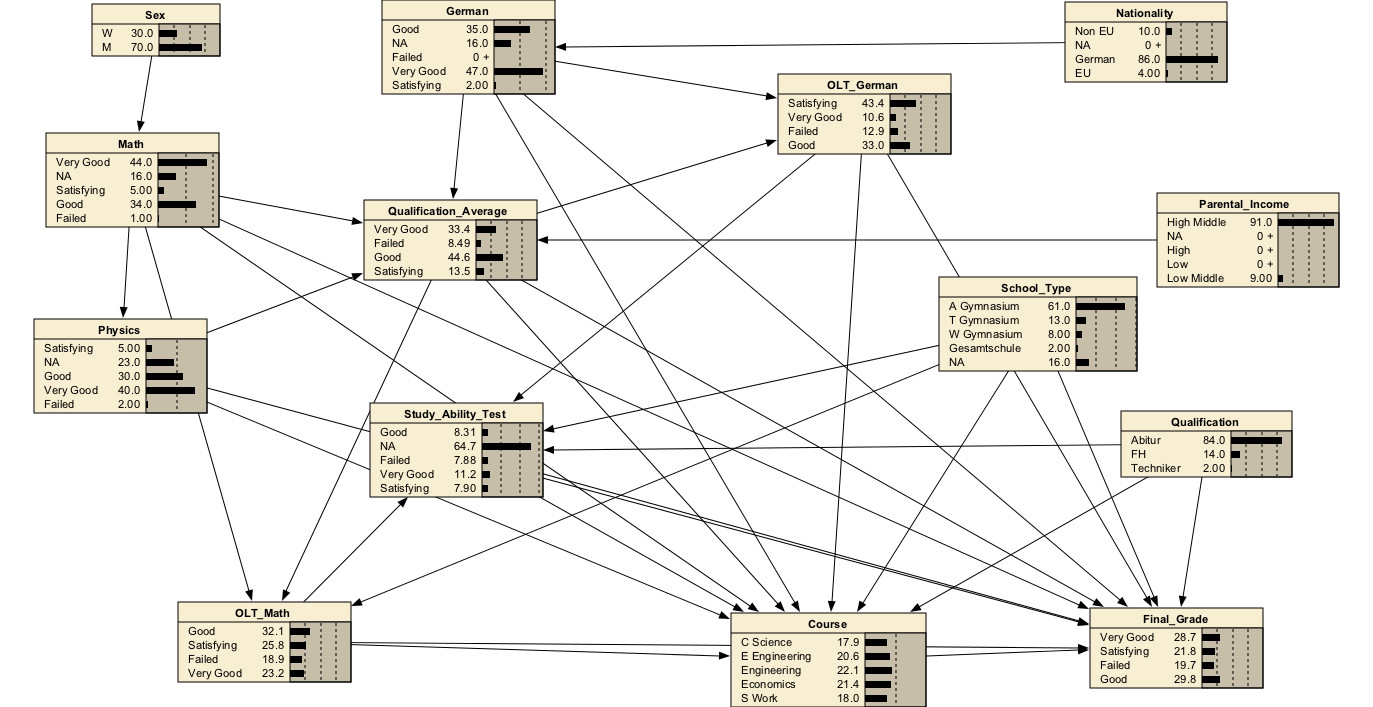
\includegraphics[width=\linewidth]{StudyNet_final_ohne_State.jpeg}
		\centering
		\caption{Finales Netz}
		\label{FinalesNetz}
	\end{figure}
\end{landscape}
  

\chapter{Learning conditional probability tables (CPT)}
To create the network we used Netica. After we made the first draw for a network and all nodes were connected in a plausible way, the CPTs needed to be calculated. Netica offers three different functions to learn the CPTs from data. After testing each of the learning algorithms, we could achieve the best results with the Expectation Maximization Algorithm.

"Briefly, E[xpectation] M[aximization] learning repeatedly takes a Bayes net and uses it to find a better one by doing an expectation (E) step followed by a maximization (M) step. In the E step, it uses regular Bayes net inference with the existing Bayes net to compute the expected value of all the missing data, and then the M step finds the maximum likelihood Bayes net given the now extended data". \cite{Netica:Online}\\
Other learning algorithms offered were counting, which is the simplest and fastest one, and gradient descent. Gradient Descent is faster than Expectation Maximization, whereas the latter one is more robust. Both perform better than counting, if there are missing values.\\
Figure \ref{Parallel} \nameref{Parallel} on the next page shows all trainings data in a parallel coordinate system. All these cases were taken into the calculation of the CPTs.

\begin{landscape}
	\begin{figure}
		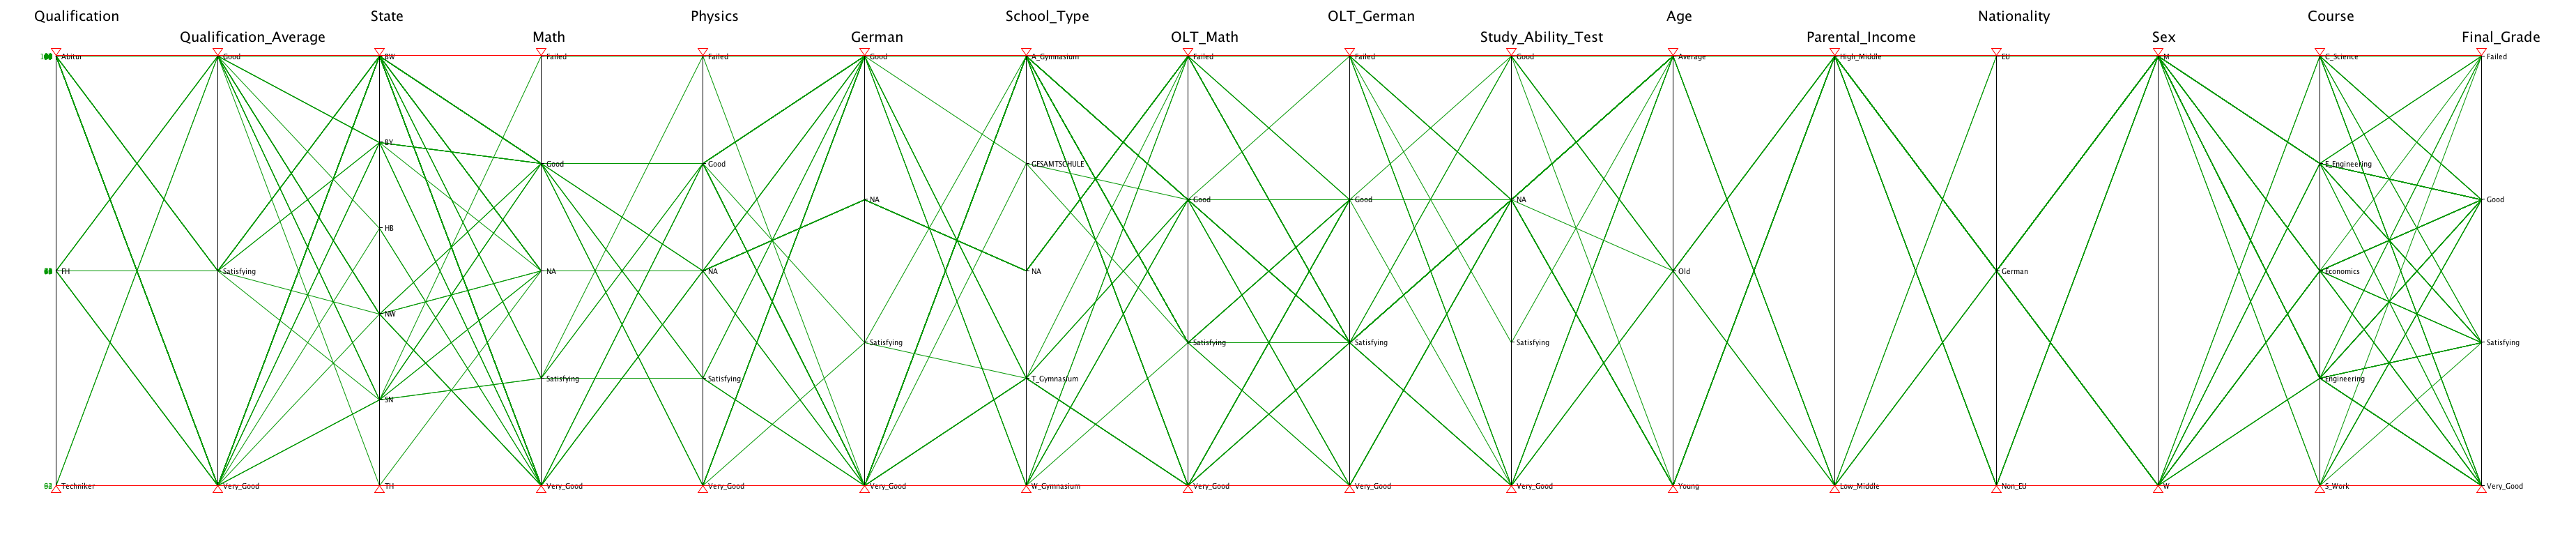
\includegraphics[width=\linewidth]{Parallel.png}
		\centering
		\caption{Parallele Koordinaten}
		\label{Parallel}
	\end{figure}
\end{landscape}


\chapter{Implementation - WhatToStudy}
Concrete implementation of the program, functionalities and documentation of implementation

%Include source code from file using:
%\lstinputlisting[caption=Expected output for the program (implemented using the Bridge design pattern)]{./Source/de/steilerdev/swe/Bridge/output}

\lstlistoflistings
\printbibliography

\begin{appendices}

%Include pdf for appendix using:
%\includepdf[pages=-,addtotoc={1,chapter,0,Exercise 1.2 - UML,app:Ex1.2-UML}]{./UML/Exercise1.pdf}

\end{appendices}

\end{document}